\documentclass[tikz,border=8pt]{standalone}
\usetikzlibrary{arrows.meta,positioning,calc}
\begin{document}
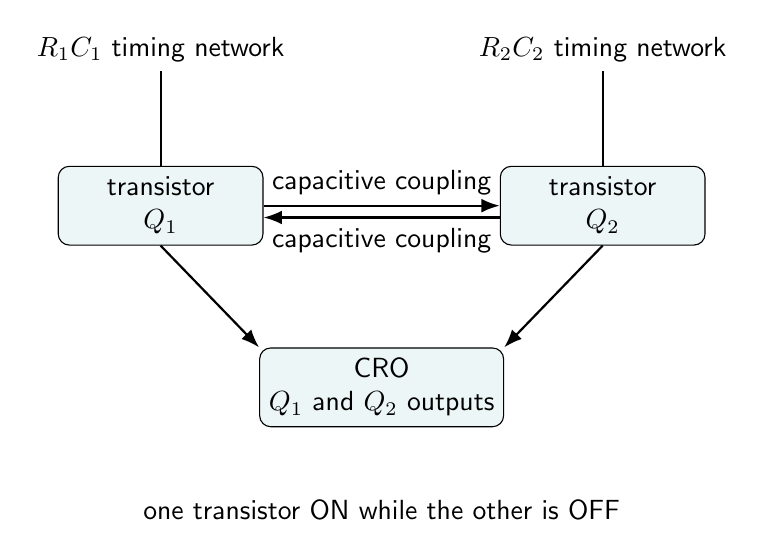
\begin{tikzpicture}[font=\sffamily,>=Latex,box/.style={draw,rounded corners,minimum height=10mm,minimum width=26mm,align=center,fill=teal!7}]
\node[box] (q1) {transistor\\$Q_1$};
\node[box,right=30mm of q1] (q2) {transistor\\$Q_2$};
\draw[thick,-Latex] (q1.east)--node[above] {capacitive coupling}(q2.west);
\draw[thick,-Latex] (q2.west |- 0,-.15)--node[below] {capacitive coupling}(q1.east |- 0,-.15);
\node[above=12mm of q1] (r1) { $R_1C_1$ timing network};
\node[above=12mm of q2] (r2) { $R_2C_2$ timing network};
\draw[thick] (q1.north)--(r1.south);
\draw[thick] (q2.north)--(r2.south);
\node[box,below=18mm of $(q1)!0.5!(q2)$] (cro) {CRO\\$Q_1$ and $Q_2$ outputs};
\draw[thick,-Latex] (q1.south)--(cro.north west);
\draw[thick,-Latex] (q2.south)--(cro.north east);
\node[below=8mm of cro] {one transistor ON while the other is OFF};
\end{tikzpicture}
\end{document}
